\clearpage
\VerdierPhysicalPageAnchor{0098}%
\begingroup
\setlength{\abovedisplayskip}{3pt plus 2pt minus 2pt}%
\setlength{\belowdisplayskip}{3pt plus 2pt minus 2pt}%
\setlength{\jot}{2pt}%
\VerdierSemanticAnchor{ch1-3-3-4-open-conclusion-continuation}
is commutative up to homotopy.
\VerdierSemanticAnchor{ch1-3-3-4-homotopy}
Choose a homotopy $a\colon fg\rightsquigarrow g'f'$. The diagram

\VerdierSemanticAnchor{ch1-3-3-4-tr1-morphism}
\begin{center}
  $D={}$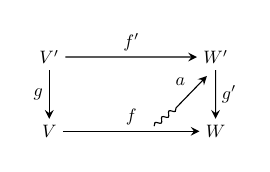
\begin{tikzpicture}[>=stealth,baseline=(current bounding box.center),
    scale=0.65,every node/.style={transform shape}]
    \node (Vp) at (0,1.45) {$V'$}; \node (Wp) at (3.25,1.45) {$W'$};
    \node (V)  at (0,0) {$V$};   \node (W)  at (3.25,0) {$W$};
    \draw[->] (Vp) -- node[above] {$f'$} (Wp);
    \draw[->] (Vp) -- node[left] {$g$} (V);
    \draw[->] (Wp) -- node[right] {$g'$} (W);
    \draw[->] (V) -- node[above] {$f$} (W);
    \draw[decorate,decoration={snake,amplitude=0.8pt,segment length=3.3pt}]
      (2.05,0.10) -- (2.48,0.46);
    \draw[->] (2.48,0.46) -- node[above left] {$a$} (3.08,1.08);
  \end{tikzpicture}
\end{center}
is a morphism of $\operatorname{tr}_1(C)$. It follows from (3.2.2.7) that
the diagram

\VerdierSemanticAnchor{ch1-3-3-4-cone-morphism-diagram}
\begin{center}
  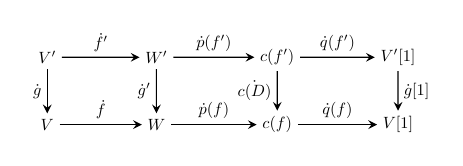
\begin{tikzpicture}[>=stealth,scale=0.59,every node/.style={transform shape}]
    \node (Vp)  at (0,1.45) {$V'$};
    \node (Wp)  at (2.35,1.45) {$W'$};
    \node (Cfp) at (4.95,1.45) {$c(f')$};
    \node (Vps) at (7.55,1.45) {$V'[1]$};
    \node (V)   at (0,0) {$V$};
    \node (W)   at (2.35,0) {$W$};
    \node (Cf)  at (4.95,0) {$c(f)$};
    \node (Vs)  at (7.55,0) {$V[1]$};
    \draw[->] (Vp) -- node[above] {$\dot f'$} (Wp);
    \draw[->] (Wp) -- node[above] {$\dot p(f')$} (Cfp);
    \draw[->] (Cfp) -- node[above] {$\dot q(f')$} (Vps);
    \draw[->] (V) -- node[above] {$\dot f$} (W);
    \draw[->] (W) -- node[above] {$\dot p(f)$} (Cf);
    \draw[->] (Cf) -- node[above] {$\dot q(f)$} (Vs);
    \draw[->] (Vp) -- node[left] {$\dot g$} (V);
    \draw[->] (Wp) -- node[left] {$\dot g'$} (W);
    \draw[->] (Cfp) -- node[left] {$\dot{c(D)}$} (Cf);
    \draw[->] (Vps) -- node[right] {$\dot g[1]$} (Vs);
  \end{tikzpicture}
\end{center}
is a morphism of triangles in $K(C)$, whence the existence of the morphism

\VerdierSemanticAnchor{ch1-3-3-4-r-conclusion}
\[
  r\colon Z'\longrightarrow Z.
\]

\VerdierSemanticAnchor{ch1-3-3-5}
\noindent\textbf{Proposition 3.3.5. (TRIV)}\quad
\begingroup\itshape
\VerdierSemanticAnchor{ch1-3-3-5-triv}
Let

\VerdierSemanticAnchor{ch1-3-3-5-input-triangle}
\begin{center}
  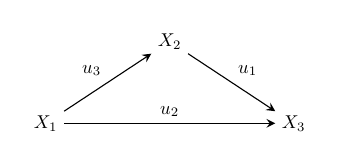
\begin{tikzpicture}[>=stealth,scale=0.67,every node/.style={transform shape}]
    \node (X1) at (0,0) {$X_1$};
    \node (X2) at (2.35,1.55) {$X_2$};
    \node (X3) at (4.70,0) {$X_3$};
    \draw[->] (X1) -- node[above left] {$u_3$} (X2);
    \draw[->] (X2) -- node[above right] {$u_1$} (X3);
    \draw[->] (X1) -- node[above] {$u_2$} (X3);
  \end{tikzpicture}
\end{center}
be a commutative diagram in $K(C)$. There exist three distinguished triangles

\VerdierSemanticAnchor{ch1-3-3-5-triangle-3}
\[
  X_1\xrightarrow{u_3}X_2\xrightarrow{v_3}Z_3
  \xrightarrow{w_3}X_1[1],
\]
\VerdierSemanticAnchor{ch1-3-3-5-triangle-1}
\[
  X_2\xrightarrow{u_1}X_3\xrightarrow{v_1}Z_1
  \xrightarrow{w_1}X_2[1],
\]
\VerdierSemanticAnchor{ch1-3-3-5-triangle-2}
\[
  X_1\xrightarrow{u_2}X_3\xrightarrow{v_2}Z_2
  \xrightarrow{w_2}X_1[1]
\]
\VerdierSemanticAnchor{ch1-3-3-5-morphisms}
and two morphisms

\VerdierSemanticAnchor{ch1-3-3-5-m1}
\[
  m_1\colon Z_3\longrightarrow Z_2,
\]
\VerdierSemanticAnchor{ch1-3-3-5-m3}
\[
  m_3\colon Z_2\longrightarrow Z_1,
\]
\VerdierSemanticAnchor{ch1-3-3-5-open-conditions}
such that:
\endgroup
\endgroup
